%!TEX root = AllegThesis.tex
%
% $Id: ch01_overview
%
\chapter{Mu2e Overview}\label{ch:overview}

\section{Background of Mu2e Experiment}
The goal of the Mu2e experiment is to detect the neutrinoless decay of a muon to an electron in the field of the nucleus. This process, if discovered, would be the first detection of Charge Lepton Flavor Violation. According to the Standard Model, the ratio ($R_{\mu e}$) of the processes:
\begin{equation}
  R_{\mu e} =  \frac{\mu^{-} + A (Z , N) \rightarrow e^{-} + A (Z,N)}{\mu^{-} + A(Z,N) \rightarrow \nu_{\mu}  + A(Z-1,N)}
\end{equation}
should be less than $10^{-50}$, a ratio undetectable by current technology. However, in several Supersymmetric Theories, this ratio can be as high as $10^{-14}$, a rate which lies within the expected range of detectability in Mu2e. Hence, the results of this experiment will either detect this phenomenon or put severe restrictions on possible theories.

For this experiment, the apparatus shown in Figure \ref{Mu2eApparatus} will be used. The rest of this paper will focus on the tracker region. 

%To achieve such levels of intensity to detect neutrinoless decays of muons to electrons, the following apparatus will be used: 

\begin{figure}[htp!]
    \centering
    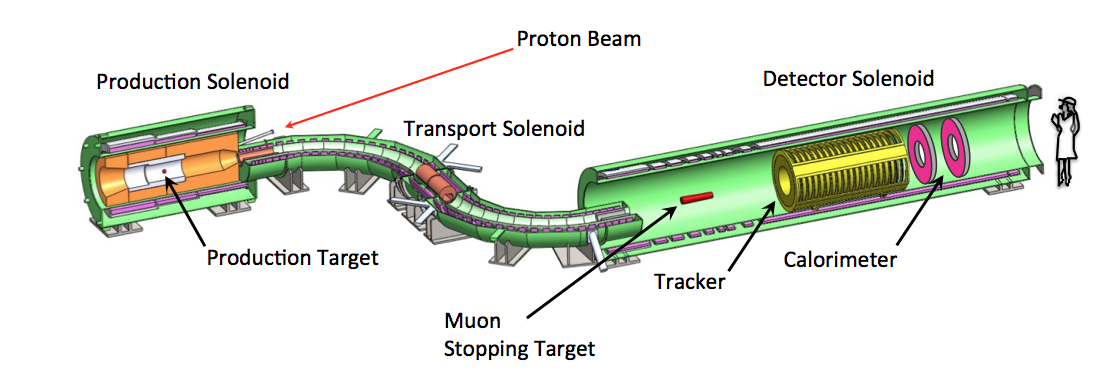
\includegraphics[width=0.8\textwidth]{Images/Mu2eDetector.png}
    \caption{Apparatus used in the Mu2e experiment}
    \label{Mu2eApparatus}
\end{figure} 

\section{Tracker}
The main purpose of the tracker is to measure the momentum of electrons with energies above 53 MeV. To accomplish this, the tracker will consist of 20,736 Mylar straw tubes ranging in length from 334 mm to 1174 mm with diameters of 5 mm. These straws will be arranged into planes which when combined form the tracker (Figure \ref{trackerSolenoid}).

\begin{figure}[htp!]
    \centering
    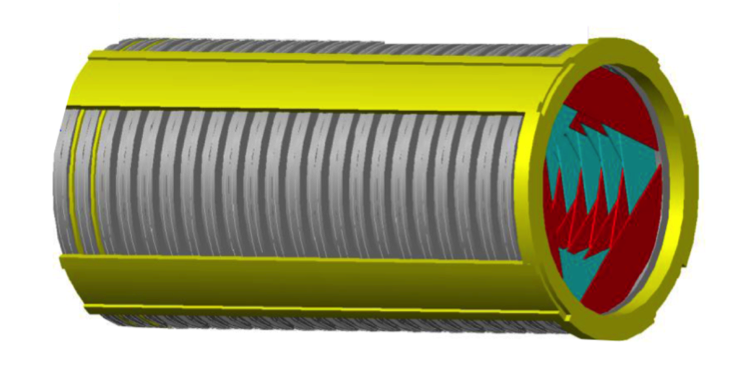
\includegraphics[width=0.55\textwidth]{Images/trackerSolenoid.png}
    \caption{Tracker solenoid.}
    \label{trackerSolenoid}
\end{figure} 

Each straw is a drift chamber such that when a particle passes through the straw, it will ionize molecules in the gas resulting in a current on the wire. This current is then passed through the straw electronics which shapes the signal to produce a voltage waveform.

By integrating the waveform from the Analog-to-Digital Converter (ADC) output, it is possible to obtain an estimate of the deposited energy. The deposited energy can then be used to differentiate particle species. In addition to muons, a major source of accidentals in the detector will be due to protons produced by nuclear breakup from muon capture. Since the average proton produced will deposit significantly more energy (roughly one order of magnitude greater) than the electrons, computing the energy from the ADC output will play a major role in differentiating these particles.

\section{Simulations}
Currently, the Mu2e collaboration has produced simulations of the tracker and the corresponding electronics. These  simulations assume the electronic response is well-approximated a high-pass RC filter followed by a low-pass CR filter to produce a voltage waveform of the form.

\begin{equation}
   V (t) = \frac{t}{\tau^2} e^{-t / \tau}
 \end{equation} 
where $V$ has been normalized. This potential is then digitized by an ADC. A sample output is shown in Figure % \ref{SampleWaveform}. 

FIXME : IMPROVE THIS

\section{Tracker Prototype}
To study the straw electronics, a prototype of the tracker has been used.
\begin{figure}[htp!]
    \centering
    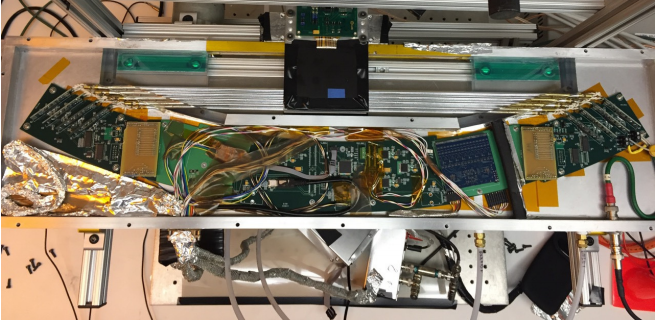
\includegraphics[width=0.55\textwidth]{Images2/prototype.png}
    \caption{Prototype of the Mu2e tracker.}
    \label{prototype}
\end{figure} 
The prototype consists of eight straws which together make up a subset of one panel (Figure \ref{prototype}). With this setup radioactive sources were pointed at the straws to produce signals that mimic what will be seen in the actual experiment. With this data we can verify and measure properties of the straw electronics, and in addition update and tune the current simulations.

 %At lower voltages the output of the simulations appear correct. However, at higher voltages corrections are clearly needed. In addition, several other electronic parameters appear to be different than the values currently implemented in the simulation. 

\section{Purpose}
The goal of the work described in this paper is twofold. First, we study the output of the tracker prototype and reconcile several results with the simulation. Second, we develop algorithms to efficiently reconstruct the energies from the waveforms. This will be key in differentiating hits from electrons and protons and determining a particle's identity.


